
 \newpage
 \section{Aim of this document}
 The goal of this document is a feasibility study to develop an automatic circuit equation
 formulation and software taking into account eventual non smooth components. It consists in including in the standard framework of SPICE piecewise linear laws  and complementarity conditions. The first part studies the modified nodal analysis(M.N.A). As a starting point, the
 MNA will be used and we will see how it is adapted to manage the non smooth components.
 \section{Notations}
\begin{itemize}
  \item[--] U is a tension, I is a current.
  \item[--] V denotes a potential at node.
  \item[--] q denotes a charge in a capacitor.
  \item[--] $\psi$ denotes a flux in a inductor.
  \item[--] Indices $_{a}$ denotes the current branch.
  \item[--] Indices $_{b}$ denotes the other branch whose voltage is a controlling variable.
  \item[--] Indices $_{c}$ denotes the other branch whose current is a controlling variable.
\item[--] CD : Current Defined
\item[--] VD : Voltage Defined
\item[--] MNA : Modify Nodal Analysis
\item[--] DAE : Differential-Algebraic Equations
\item[--] MLCP : Mixed Linear Complementarity Problem.
\item[--] $N_{I}$ : Number of unknowns.
\item[--] $N_{E}$ : Number of equations.
\item[--] $I_{j}$ : Current in the branch number j.
\item[--] $V_{i}$ : Voltage on node number i.
\end{itemize}
\include{StandardMNA}
\section{The linear non smooth components}
\subsection{Topology. Choice of smooth and nonsmooth components.}
The stamp method is used for the linear components. About the non smooth components, a piecewise
linear modeling describes the component's behavior. This geometry is written with linear
complementarity conditions. 
\subsection{Unknowns}
Before go head, the unknowns vector X is subdivided:
\begin{enumerate}
\item[--] x contains only the dynamic unknowns(currents in inductor and tensions from capacitor branches)
\item[--] $Z_{s}$ contains only the non dynamic unknowns(Voltage nodes,... ).
\item[--] $Z_{ns}$ contains the useful currents and tensions for the non smooth components.
\end{enumerate}
\subsection{Linear local formulation}
For each non smooth component, we assume that the behavior can be written as the following the mixed linear  complementarity condition, that is:
\begin{equation}\left(\begin{array}{c}
\beta = Z_{nsi} = A_{i}x+B_{i}\lambda_{i}+C_{i}Z_{s} + a_{i}\\
y_{i}=D_{i}x+E_{i}Z_{s}+F_{i}\lambda_{i}+G_{i}Z_{nsi}+e_{i}\\
0 \leq y_{i} \, \perp \, \lambda_{i} \geq 0
\end{array}\right)
\end{equation}
where $Z_{nsi}$ is a voltage and currents vector. $a_{i},e_{i},\lambda_{i}$ and $y_{i}$ are some constants vectors which characterizes the components. At the end
of this document, we will see how ideal diode and piecewise linear models of transistor fits into this formulation.


\subsection{Example of a linear global formulation}
It consists in writing all the complementary conditions in the equations of the MNA. An example with 5 non smooth components is given by:

\[\left(\begin{array}{c}
  Z_{ns}\\
  \hline
  Z_{ns1} \\
  Z_{ns2} \\
  Z_{ns3} \\
  Z_{ns4} \\
  Z_{ns5} \\
\end{array}\right) =
\left(\begin{array}{c}
  C_{1x}\\
  \hline
  A1\\
  A2\\
  A3\\
  A4\\
  A5\\
\end{array}\right)*x +
\left(\begin{array}{c}
  C_{1s}\\
  \hline
  C1\\
  C2\\
  C3\\
  C4\\
  C5\\
\end{array}\right)*Z_{s} +
\left(\begin{array}{ccccc}
  C1_{\lambda}\\
  \hline
  B1&0&0&0&0\\
  0&B2&0&0&0\\
  0&0&B3&0&0\\
  0&0&0&B4&0\\
  0&0&0&0&B5\\
\end{array}\right)*
\left(\begin{array}{c}
  \lambda\\
  \hline
  \lambda _{1} \\
  \lambda _{2}\\
  \lambda _{3}\\
  \lambda _{4}\\
  \lambda _{5}\\
\end{array}\right)+
\left(\begin{array}{c}
  cst\\
  \hline
   cst_{1} \\
   cst_{2}\\
   cst_{3}\\
   cst_{4}\\
   cst_{5}\\
\end{array}\right)
\]

\[\left(\begin{array}{c}
  Y\\
  \hline
   Y_{1} \\
   Y_{2} \\
   Y_{3} \\
   Y_{4} \\
   Y_{5} \\
\end{array}\right) =
\left(\begin{array}{c}
  D_{1x}\\
  \hline
  D1\\
  D2\\
  D3\\
  D4\\
  D5\\
\end{array}\right)*x +
\left(\begin{array}{c}
  D_{1s}\\
  \hline
  E1\\
  E2\\
  E3\\
  E4\\
  E5\\
\end{array}\right)*Z_{s} +
\left(\begin{array}{ccccc}
  D1_{\lambda}\\
  \hline
  F1&0&0&0&0\\
  0&F2&0&0&0\\
  0&0&F3&0&0\\
  0&0&0&F4&0\\
  0&0&0&0&F5\\
\end{array}\right)*
\left(\begin{array}{c}
  \lambda\\
  \hline
   \lambda _{1} \\
   \lambda _{2}\\
   \lambda _{3}\\
   \lambda _{4}\\
   \lambda _{5}\\
\end{array}\right)+\]
\[
\left(\begin{array}{ccccc}
  D1_{ns}\\
  \hline
  G1&0&0&0&0\\
  0&G2&0&0&0\\
  0&0&G3&0&0\\
  0&0&0&G4&0\\
  0&0&0&0&G5\\
\end{array}\right)*
\left(\begin{array}{c}
  Zns\\
  \hline
   Z_{ns1} \\
   Z_{ns2}\\
   Z_{ns3}\\
   Z_{ns4}\\
   Z_{ns5}\
\end{array}\right)+
\left(\begin{array}{c}
  cst\\
  \hline
   cst_{1} \\
   cst_{2}\\
   cst_{3}\\
   cst_{4}\\
   cst_{5}\\
\end{array}\right)
\]
Finally, the global formulation form is : 

\[\left(\begin{array}{c}
Z_{ns}= C_{1x}x+C_{1zs}Z_{s}+C_{1\lambda}\lambda +C_{1s}\\
Y=D_{1x}x +D_{1zs}Z_{s}+D_{1ns}Z_{ns}+D_{1\lambda}\lambda+D_{1s}\\
0 \leq Y \, \perp \, \lambda \geq 0
\end{array}\right)\]
\newpage
\section{Extended MNA for nonsmooth linear components}
This part describes the automatic formulation into a Mixed Linear Complementarity System (MLCS) of a circuit. It consists in adapting the MNA to manage non-smooth model.

\subsection{MLCS and MLCP definitions}
\begin{definition}\index{Complementarity problem ! mixed linear} \index{MLCP}
  Given the matrices  ${A} \in \RR^{n \times n}$, ${B} \in \RR^{m \times m}$, ${C} \in \RR^{n \times m}$, ${D} \in \RR^{m \times n}$, and the vectors  $ {a} \in \RR^n, {b} \in \RR^m$, the MLCP denoted by $\mathrm{MLCP}(A,B,C,D,a,b)$ consists in finding two vectors $ {u} \in \RR^n$ and  $ {v} \in \RR^m$ such that
\begin{equation}\label{eq:mlcp1} 
  \begin{cases}
    A u + C v + a =0 \\  \\
    {0} \le {v} \perp     Du +B v +b   \ge {0}
  \end{cases}.
\end{equation}
The  MLCP can be defined equivalently in the following form denoted by $\mathrm{MLCP}(M,q,\mathcal E,\mathcal I)$
\begin{equation}
  \label{eq:mlcp2}
  \begin{cases}
    w = M z +q \\
    w_i=0,\forall  i \in \mathcal E \\
    {0} \le z_i \perp w_i \ge {0}, \forall  i \in \mathcal I 
 \end{cases}
\end{equation}
where  $\mathcal E$ and $\mathcal I$ are finite sets of indices such that $\mathrm{card}(\mathcal E \cup \mathcal I  ) = n$ and $\mathcal E \cap \mathcal I  = \emptyset$.\end{definition}
The MLCP is a mixture between an LCP and a system of linear equations. The former definition~(\ref{eq:mlcp1}) can be casted into the second one~(\ref{eq:mlcp2}) by introducing
\begin{equation}
  \label{eq:mlcp-m}
  M = \left[
  \begin{array}{cc}
   A & C \\
   D & B
  \end{array}\right],\quad   q = \left[
  \begin{array}{c}
    a \\
    b
  \end{array}\right],\quad   z = \left[
  \begin{array}{c}
    u \\
    v
  \end{array}\right],\quad   w = \left[
  \begin{array}{c}
    0\\
    w_i, \forall  i \in \mathcal I 
  \end{array}\right]
\end{equation}




Equivalently, the MLCS can be defined by an implicit system

\begin{definition}\index{Complementarity system ! mixed linear} \index{MLCS}
  Given the matrices  ${M} \in \RR^{n \times n}$, ${A} \in \RR^{n \times n}$, ${B} \in \RR^{m \times
  m}$, ${C} \in \RR^{n \times m}$, ${D} \in \RR^{m \times n}$, and the vectors  $ {a} \in \RR^n, {b}
  \in \RR^m$, the implicit MLCS denoted by $\mathrm{IMLCS}(M,A,B,C,D,a,b)$ consists in finding two vectors $ {x} \in \RR^n$ and  $ {v} \in \RR^m$ such that
\begin{equation}\label{eq:mlcs1} 
  \begin{cases}
   M x' = A x + C v + a  \\  \\
   {0} \le {v} \perp     Dx +B v +b   \ge {0}
  \end{cases}.
\end{equation}
\end{definition}

or an explicit system
\begin{definition}\index{Complementarity system ! mixed linear} \index{MLCS}
  Given the matrices   ${A_{x}} \in \RR^{n \times n}$, ${A_{z}} \in \RR^{n \times
  p}$, ${A_{v}} \in \RR^{n \times m}$, ${B_{x}} \in \RR^{p \times n}$, ${B_{z}} \in \RR^{p \times
  p}$, ${B_{v}} \in \RR^{p \times m}$, ${C_{x}} \in \RR^{m \times n}$, ${C_{z}} \in \RR^{m \times p}$,${C_{v}} \in \RR^{m \times m}$, and
  the vectors  $ {a} \in \RR^n$,$ {b}  \in \RR^p$,$ {c}  \in \RR^m$, the explicit MLCS denoted by
  $\mathrm{EMLCS}(A_{x},A_{z},A_{v},B_{x},B_{z},B_{v},C_{x},C_{z},C_{v},a,b,c)$ consists in finding three vectors $ {x}
  \in \RR^n$, $ {z} \in \RR^p$ and  $ {v} \in \RR^m$ such that
\begin{equation}\label{eq:mlcs2} 
  \begin{cases}
   x' = A_{x} x +A_{z} z +A_{v} v + a  \\
   0 = B_{x} x +B_{z} z + B_{v} v +b \\ \\
   {0} \le {v} \perp     C_{x} x+ C_{z}z +C_{v} v +c   \ge {0}
  \end{cases}.
\end{equation}
\end{definition}
\subsection{Hypothesis}
The MNA assumes smooth branches are explicit functions of current or voltage. It means each smooth
branch is Voltage Defined (V.D.) or Current Defined (C.D.)\\

With the same assumption, all branches can be divided into following classes:\\
\begin{enumerate}
\item The  \underline{C.D. branches} 
\item The  \underline{V.D. branches}
 \item The  \underline{non smooth branches}
 \item The \underline{dynamical capacitor branches}
 \item The \underline{dynamical inductors branches}
\end{enumerate}




\subsection{Nonsmooth equations and MLCS}
With the linear complementary condition, the system becomes an explicit MLCS of the form :
\[x' = A_{1x}x +A_{1zs}Z_{s} + A_{1ns}Z_{ns}+A_{1s}\]
\[0  = B_{1x}x+B_{1zs}Z_{s} + B_{1ns}Z_{ns}+B_{1s}\]
\[Z_{ns}= C_{1x}x+C_{1zs}Z_{s}+C_{1\lambda}\lambda +C_{1s}\]
\[Y=D_{1x}x +D_{1zs}Z_{s}+D_{1ns}Z_{ns}+D_{1\lambda}\lambda+D_{1s}\]
\[0 \leq Y \, \perp \, \lambda \geq 0\]
 

\section{How get $x' = A_{1x}x +A_{1zs}Z_{s} + A_{1ns}Z_{ns}+A_{1s}$?}
To get this system, a good set of unknowns must be done. Only the necessary unknowns are added. The
following examples show how this choice could be done.
\subsection{Example 1}
\begin{figure}[h]
\centerline{
 \scalebox{0.5}{
    \input{../ace/cir1.pstex_t}
 }
}
\end{figure}
\paragraph{First matrices formulation}
X=$^{t}(V_{1},V_{2},V_{3})$\\
\[\left(\begin{array}{c}
  \\
  KCL(1)\\  KCL(2)\\  KCL(3)
  \end{array}\right)
\left(\begin{array}{ccc}
  V_{1}&V_{2}&V_{3}\\
  \hline
  \frac{1}{R}-\frac{1}{R}&  \frac{-1}{R}&0\\
  \frac{1}{R}&  \frac{-1}{R}&0\\
  0&0&\frac{1}{R}
\end{array}\right)X+
\underline{
\left(\begin{array}{ccc}
   V_{1}'&V_{2}'&V_{3}'\\
  \hline
0&0&0\\
  0&C&-C\\
  0&-C&C
\end{array}\right)}X'=
\left(\begin{array}{c}
  \\
  I\\
  0\\
  0
  \end{array}\right)
\]
But, we can't extract x from X to get x'=...\\
\newline
\paragraph{Add current and tension from the capacitor}
x=$(U_{32})$
$Z_{s}=^{t}(V_{1},V_{2},V_{3},I_{32})$\\
\[x'=CI_{32}\]
\[\left(\begin{array}{c}
  \\
  KCL(1)\\
  KCL(2)\\
  KCL(3)\\
  U_{32}
  \end{array}\right)
\left(\begin{array}{cccc}
  V_{1}&V_{2}&V_{3}&I_{32}\\
  \hline
  \frac{1}{R}-\frac{1}{R}&  \frac{-1}{R}&0&0\\
  \frac{1}{R}&  \frac{-1}{R}&0&1\\
  0&0&\frac{1}{R}&-1\\
  0&-1&1&0
\end{array}\right)Z_{s}+
\left(\begin{array}{c}
  U_{32}\\
  \hline
  0\\
  0\\
  0\\
  1
  \end{array}\right)x
=
\left(\begin{array}{c}
  \\
  I\\
  0\\
  0\\
  0
  \end{array}\right)
\]
We obtain the matrices system\\
\[x'=A1_{zs}Z_{s}\]
\[Ax+CZ_{s}=s\]
$N_{I}=N_{E}=5$\\
The following examples, show we don't need to add the capacitor current. Sometime, current in
capacitor can be replace with a KCL law.\\

\paragraph{Add only tension from the capacitor}
x=$(U_{32})$,$Z_{s}=^{t}(V_{1},V_{2},V_{3})$\\
First get x' with \underline{KCL(3)}:
\[x'=\frac{V_{3}}{RC}\]
Second, the current in capacitor is $\frac{V_{3}}{R}$, and use it to write other KCL law:
\[\left(\begin{array}{c}
  \\
  KCL(1)\\
  KCL(2)\\
  U_{32}
  \end{array}\right)
\left(\begin{array}{ccc}
V_{1}&V_{2}&V_{3}\\
  \hline
  \frac{1}{R}+\frac{1}{R}&  \frac{-1}{R}&0\\
  \frac{-1}{R}&  \frac{1}{R}&\frac{1}{R}\\
  0&-1&1
\end{array}\right)Z_{s}+
\left(\begin{array}{c}
U_{32}\\
  \hline
  0\\
  0\\
  0\\
  1
  \end{array}\right)x
=
\left(\begin{array}{c}
  \\
  I\\
  0\\
  0\\
  0
  \end{array}\right)
\]
$N_{I}=N_{E}=4$
\newpage

 
\subsubsection{Example 2}
\begin{figure}[h]
\centerline{
 \scalebox{0.9}{
    \input{cir2.pstex_t}
 }
}
\end{figure}
\paragraph{Add currents and tensions from the capacitor}
$x=^{t}(I_{42},U_{43},U_{31},U_{50})$,
$Z_{s}=^{t}(V_{1},V_{2},V_{3},V_{4},V_{5},I_{43},I_{31},I_{50})$
We obtain following equation:
\[\left(\begin{array}{cccc}
  I_{42}'&U_{43}'&U_{31}'&U_{50}'\\
  \hline
L&0&0&0\\
0&C&0&0\\
0&0&C&0\\
0&0&0&C
\end{array}\right)x'=
0x+
\left(\begin{array}{cccccccc}
  V_{1}&V_{2}&V_{3}&V_{4}&V_{5}&I_{43}&I_{31}&I_{50}\\
  \hline
  0&1&0&-1&0&0&0&0\\
  0&0&0&0&0&-1&0&0\\
  0&0&0&0&0&0&1&0\\
  0&0&0&0&0&0&0&1\\
\end{array}\right)Z_{s}
\]
\[\left(\begin{array}{c}
\\KCL(1)\\KCL(2)\\KCL(3)\\KCL(4)\\KCL(5)\\U_{43}\\U_{31}\\U_{50}
\end{array}\right)
\left(\begin{array}{cccccccc}
  V_{1}&V_{2}&V_{3}&V_{4}&V_{5}&I_{43}&I_{31}&I_{50}\\
  \hline
  -\frac{1}{R}&\frac{1}{R}&0&0&0&0&1&0\\
  \frac{1}{R}&-\frac{1}{R}&0&0&0&0&0&0\\
  0&0&0&0&0&-1&1&0\\
  0&0&0&-\frac{1}{R}&\frac{1}{R}&1&0&0\\
  0&0&0&\frac{1}{R}&-\frac{1}{R}&0&0&1\\
  0&0&-1&1&0&0&0&0\\
  -1&0&1&0&0&0&0&0\\
  0&0&0&0&1&0&0&0\\
\end{array}\right)Z_{s}+
\left(\begin{array}{cccc}
  I_{42}&U_{43}&U_{31}&U_{50}\\
  \hline
  0&0&0&0\\
  1&0&0&0\\
  0&0&0&0\\
  0&0&0&0\\
  1&0&0&0\\
  0&1&0&0\\
  0&0&1&0\\
  0&0&0&1\\
\end{array}\right)x=
\left(\begin{array}{c}
  \\ I\\  0\\  0\\  0\\  0\\  0\\  0\\  0
  \end{array}\right)
\]

\[x'=A1_{zs}Z_{s}\]
\[Cx+BZ_{s}=s\]
$N_{I}=N_{E}=12$
\paragraph{Add only tensions from the capacitor}
$x=^{t}(I_{42},U_{43},U_{31},U_{50})$,
$Z_{s}=^{t}(V_{1},V_{2},V_{3},V_{4},V_{5})$\\
We obtain following equation:
\[
\left(\begin{array}{c}
  \\  KCL(4)\\  KCL(3)\\  KCL(5)
\end{array}\right)
\underline{
\left(\begin{array}{cccc}
  I_{42}'&U_{43}'&U_{31}'&U_{50}'\\
  \hline
L&0&0&0\\
0&C&0&0\\
0&C&C&0\\
0&0&0&C
\end{array}\right)}x'=
\left(\begin{array}{cccc}
  I_{42}&U_{43}&U_{31}&U_{50}\\
  \hline
0&0&0&0\\
1&0&0&0\\
0&0&0&0\\
0&0&0&0\\ 
\end{array}\right)x+
\left(\begin{array}{ccccc}
V_{1}&V_{2}&V_{3}&V_{4}&V_{5}\\
  \hline
  0&1&0&-1&0\\
  0&0&0&\frac{1}{R}&-\frac{1}{R}\\
  0&0&0&0&0\\
  0&0&0&-\frac{1}{R}&\frac{1}{R}
\end{array}\right)Z_{s}
\]
So, we get $x'=A1_{x}x+A1_{zs}Z_{s}$. Therefore, all currents in the capacitor branch are known.\\
$I_{43}= I_{42}+\frac{V_{4}}{R}-\frac{V_{5}}{R}$,
$I_{31}= I_{42}+\frac{V_{4}}{R}-\frac{V_{5}}{R}$,
$I_{50}= \frac{V_{4}}{R}-\frac{V_{5}}{R}$\\
Use these equations to fill following matrices:
\[\left(\begin{array}{c}
KCL(1)\\KCL(2)\\U_{43}\\U_{31}\\U_{50}
\end{array}\right)
\left(\begin{array}{ccccc}
V_{1}&V_{2}&V_{3}&V_{4}&V_{5}\\
  \hline
  -\frac{1}{R}&\frac{1}{R}&0&\underline{\frac{1}{R}}&\underline{-\frac{1}{R}}\\
  \frac{1}{R}&-\frac{1}{R}&0&0&0\\
  0&0&-1&1&0\\
  -1&0&1&0&0\\
  0&0&0&0&1\\
\end{array}\right)Z_{s}+
\left(\begin{array}{cccc}
  I_{42}&U_{43}&U_{31}&U_{50}\\
  \hline
  \underline{1}&0&0&0\\
  1&0&0&0\\0&1&0&0\\0&0&1&0\\0&0&0&1\\
\end{array}\right)x=
\left(\begin{array}{c}
  I\\0\\0\\0\\0
  \end{array}\right)
\]
$N_{I}=N_{E}=9$


\subsection{Example 3}
\begin{figure}[h]
\centerline{
 \scalebox{0.8}{
    \input{cir3.pstex_t}
 }
}
\end{figure}

x=$(U_{12})$\\
$Z_{s}=^{t}(V_{1},V_{2},I_{10})$\\
\[(KCL(1))=>(C1+C2+C3)x'=I_{10}\]
So, all capacitor's currents are known:\\
$I_{c1}=\frac{C1}{C1+C2+C3}I_{10}$\\
$I_{c2}=\frac{C2}{C1+C2+C3}I_{10}$\\
$I_{c3}=\frac{C3}{C1+C2+C3}I_{10}$\\
Use these equations to fill following matrices:\\
\[\left(\begin{array}{c}
  \\
KCL(2)\\U_{21}\\VD
\end{array}\right)
\left(\begin{array}{c}
U_{21}\\
\hline
0\\
1\\
0
\end{array}\right)x+
\left(\begin{array}{ccc}
V_{1}&V_{2}&I_{10}\\
\hline
0&\frac{1}{R}&\frac{C1}{C1+C2+C3}+\frac{C2}{C1+C2+C3}+\frac{C3}{C1+C2+C3}\\
1&-1&0\\
1&0&0
\end{array}\right)Z_{s}=
\left(\begin{array}{c}
\\0\\0\\E
\end{array}\right)
\]
$N_{I}=N_{E}=4$
\newpage

\subsection{Example 4}
This example shows that is not always possible to use the KCL law to get x'=...\\
\begin{figure}[h]
\centerline{
 \scalebox{0.9}{
    \input{cir4.pstex_t}
 }
}\end{figure}\\
$x=^{t}(U_{21},U_{23},U_{34})$
$Z_{s}=^{t}(V_{1},V_{2},V_{3},V_{4})$
\paragraph{a problem:}
Start to fill the x' matrices. We use KCL(2) for $U_{21}$, and KCL(3) for $U_{34}$.
\[\left(\begin{array}{c}
  \\
KCL(2)\\KCL(3)\\??
\end{array}\right)
\left(\begin{array}{ccc}
  U_{21}'&U_{23}'&U_{34}'\\
  \hline
  C&-C&0\\
  0&C&C\\
  ?&?&?
\end{array}\right)x'=0x+
\left(\begin{array}{cccc}
  V_{1}&V_{2}&V_{3}&V_{4}\\
  \hline
  0&0&0&0\\
  0&0&0&0\\
  ?&?&?&?\\
\end{array}\right)Z_{s}
 \]
 We can't use a other KCL law to get $U_{23}$. A solution could be to add an unknown, \underline{$I_{23}$} in
 $Z_{s}$. The system becomes:\\
 \[\left(\begin{array}{c}
  \\
KCL(2)\\KCL(3)\\I_{23}
\end{array}\right)
\left(\begin{array}{ccc}
  U_{21}'&U_{23}'&U_{34}'\\
  \hline
  C&-C&0\\
  0&C&C\\
  0&C&0
\end{array}\right)x'=0x+
\left(\begin{array}{ccccc}
  V_{1}&V_{2}&V_{3}&V_{4}&\underline{I_{23}}\\
  \hline
  0&0&0&0&0\\
  0&0&0&0&0\\
  0&0&0&0&1\\
\end{array}\right)Z_{s}
 \]
 So, we obtain $x'=A1_{zs}Z_{s}$. All capacitor's currents are known:
 $I_{21}=\underline{I_{23}}=I_{34}$\\
\[\left(\begin{array}{c}
  \\
KCL(4)\\KCL(1)\\U_{21}\\U_{23}\\U_{34}
\end{array}\right)
\left(\begin{array}{ccc}
  U_{21}&U_{23}&U_{34}\\
  \hline
  0&0&0\\
  0&0&0\\
  1&0&0\\
  0&1&0\\
  0&0&1
\end{array}\right)x+
\left(\begin{array}{cccc}
  V_{1}&V_{2}&V_{3}&\underline{I_{23}}\\
  \hline
  0&0&0&1\\
  \frac{1}{R}&0&0&1\\
  -1&1&0&0\\
  0&-1&1&0\\
  0&0&-1&1\\
\end{array}\right)Z_{s}=
\left(\begin{array}{c}
\\I\\0\\0\\0\\0
\end{array}\right)
\]
 $N_{I}=N_{E}=8$\\
\paragraph{a good choice:}
\[\left(\begin{array}{c}
  \\
KCL(1)\\KCL(2)\\KCL(3)
\end{array}\right)
\left(\begin{array}{ccc}
  U_{21}'&U_{23}'&U_{34}'\\
  \hline
  C&0&0\\
  C&C&0\\
  0&-C&C
\end{array}\right)x'=0x+
\left(\begin{array}{cccc}
  V_{1}&V_{2}&V_{3}&V_{4}\\
  \hline
  \frac{1}{R}&-\frac{1}{R}&0&0\\
  0&0&0&0\\
  0&0&0&0\\
\end{array}\right)Z_{s}
 \]
 So, we obtain $x'=A1_{zs}Z_{s}$. Therefore all capacitor's currents are known: $I_{12}=I_{23}=I_{34}=\frac{V1}{R1}$\\
 \[\left(\begin{array}{c}
  \\
KCL(4)\\U_{21}\\U_{23}\\U_{34}
\end{array}\right)
 \left(\begin{array}{ccc}
  U_{21}&U_{23}&U_{24}\\
  \hline
  0&0&0\\
  1&0&0\\
  0&1&0\\
  0&0&1\\
\end{array}\right)x+
 \left(\begin{array}{cccc}
  V_{1}&V_{2}&V_{3}&V_{4}\\
  \hline
  \frac{1}{R}&0&0&0\\
  -1&1&0&0\\
  0&-1&1&0\\
  0&0&-1&1\\
\end{array}\right)Z_{s}=
 \left(\begin{array}{c}
  \\I\\0\\0\\0
\end{array}\right)
 \]
$N_{I}=N_{E}=7$\\






 
\subsection{One  example with  a capacitor  loop}

\begin{ndrva}
  Mettre a jour les notations.


   Z_s --> z

   A --> M
\end{ndrva}


This example shows we have to manage the capacitor cycle.\\
\begin{figure}[h]
\centerline{
 \scalebox{0.6}{
    \input{../ace/cir5.pstex_t}
 }
}\end{figure}\\


\paragraph{Standard MNA Algorithm}
 \texttt{texte ::} $x=^{t}(U_{12},U_{23},U_{34},U_{41})$$Z_{s}=(V_{1},V_{2},V_{3},V_{4},V_{5},I_{50})$\\
Start to write Ax'=...\
\[\left(\begin{array}{c}
  \\
KCL(1)\\KCL(2)\\KCL(3)\\KCL(4)
\end{array}\right)
\left(\begin{array}{cccc}
  U_{12}'&U_{23}'&U_{34}'&U_{41}'\\
  \hline
  C&0&0&-C\\
  -C&C&0&0\\
  0&-C&C&0\\
  0&0&-C&C\\  
\end{array}\right)x'= RHS
\]
where the Right-hand-side  $RHS$ is not here detailed.
This matrix is not regular because of the cycle \{1-2,2-3,3-4,4-1\}. 



\paragraph{The proposed Algorithm \ref{Algo:}}

A solution could be to use the Minimum
Spanning Tree \{1-2,2-3,3-4\} to write the KCL law. About the last tension, $U_{41}$, there are tow
ways:
\begin{enumerate}
\item add a unknown $I_{41} in Z_{S}$ and write CU'=I
\item Find the linear relation $U_{41}'= \sum_{jk}^{}a_{jk}U_{kj}'$, and replace $U_{ki}'$.
\end{enumerate}
The matrices become:\\
Start to write Ax'=...\
\[\left(\begin{array}{c}
  \\
KCL(1)\\KCL(2)\\KCL(3)\\I_{41}
\end{array}\right)
\left(\begin{array}{cccc}
  U_{12}'&U_{23}'&U_{34}'&U_{41}'\\
  \hline
  C&0&0&-C\\
  -C&C&0&0\\
  0&-C&C&0\\
  0&0&0&C\\  
\end{array}\right)x'=0x+
\left(\begin{array}{ccccccc}
  V_{1}&V_{2}&V_{3}&V_{4}&V_{5}&I_{50}&I_{41}\\
  \hline
  -\frac{1}{R}&0&0&0&0&0&0\\
  0&0&0&0&0&0&0\\
  0&0&0&\frac{1}{R}&-\frac{1}{R}&0&0\\
  0&0&0&0&0&0&1\\
\end{array}\right)Z_{s}
\]
So, we obtain $x'=A1_{zs}Z_{s}$. Therefore all capacitor's currents are
known:$I_{12}=I_{23}=I_{41}+\frac{V1}{R},I_{43}=I_{41}+\frac{V1}{R}+\frac{V5}{R}-\frac{V3}{R}$\\
The last step consists in writing the missing equations:
 \[\left(\begin{array}{c}
  \\
KCL(4)\\KCL(5)\\U_{12}\\U_{23}\\U_{34}\\U_{41}\\VD_{50}
\end{array}\right)
 \left(\begin{array}{cccc}
  U_{12}&U_{23}&U_{34}&U_{41}\\
  \hline
  0&0&0&0\\
  0&0&0&0\\
  1&0&0&0\\
  0&1&0&0\\
  0&0&1&0\\
  0&0&0&1\\
  0&0&0&0\\

\end{array}\right)x+
 \left(\begin{array}{ccccccc}
  V_{1}&V_{2}&V_{3}&V_{4}&V_{5}&I_{50}&I_{41}\\
  \hline
  \frac{1}{R}&0&-\frac{1}{R}&0&\frac{1}{R}&0&\underline{-1+1}\\
  0&0&\frac{1}{R}&0&-\frac{1}{R}&-1&0\\
  -1&1&0&0&0&0&0\\
  0&-1&1&0&0&0&0\\
  0&0&-1&1&0&0&0\\
  0&0&0&-1&1&0&0\\
  0&0&0&0&1&0&0\\
\end{array}\right)Z_{s}=
 \left(\begin{array}{c}
  \\0\\0\\0\\0\\0\\0\\E
\end{array}\right)
 \]
$N_{I}=N_{E}=11$\\



\subsection{conclusion}
The vector x contains inductor's currents and capacitor's tensions. Derivate inductor's current is equal to a
nodal voltage difference.\\
About the capacitor's tensions, we use the Minimum Spanning Tree of the capacitor' tension to avoid cycle.\\


\begin{algorithm}
\caption{fill the matrices : $x'=A_{1x}x+A_{1s}Z_{s}+A_{1ns}Z_{ns}$ }
\begin{algorithmic}
\REQUIRE Init\_I\_in\_x : initialize internal data structure to get all I from x.
\REQUIRE Next\_I\_in\_x : return the next available I from x. If there are not available x, return 0.\\
\REQUIRE Minimum Spanning Tree of the capacitor' tension graph
\REQUIRE Init\_MST : initialize internal data structure to get all u from x.
\REQUIRE Next\_u\_in\_MST : return a available U's neighbour from MST if possible. If there are not
available u in MST, return 0.\\
\REQUIRE Next\_U\_in\_x : return the next available U from x. If there are not available x, return 0.\\

0\\
\COMMENT{About current}\\
\COMMENT{get first current}
\STATE Init\_I\_in\_x()
\STATE $I_{kj}$ = Next\_I\_in\_x()
\WHILE{$I_{kj}$}
\STATE use $LI'=V_{j}-V_{k}$ to fill $I_{kj}$'s line.
\ENDWHILE\\
\COMMENT{About tension}\\
\COMMENT{get a first capacitor tension}
\STATE Init\_MST()
\STATE $U_{kj}$ = Next\_u\_in\_MST()
\WHILE{$U_{kj}$}
\STATE l=j or k with KCL(k) available.
\STATE Use CU'=I and KCL(k) to fill $U_{ki}$'s line.\\
\STATE enable KCL(k)

\STATE $U_{kj}$= Next\_u\_in\_MST ()
\ENDWHILE
\STATE $U_{kj}$ = Next\_U\_in\_x()
\WHILE {$U_{kj}$}
\STATE Add an unknown $I_{kj}$, and use it to fill the matrices. Write I=CU'.
\STATE $U_{kj}$ = Next\_U\_in\_x()
\ENDWHILE
\COMMENT{reverse A : $Ax'=Bx+CZ_{s}+DZ_{ns}$\\}
\STATE $A^{-1}$=Inv(A)
\STATE $x'=A_{1x}x+A_{1s}Z_{s}+A_{1ns}Z_{ns}$
\end{algorithmic}
\end{algorithm}


\newpage

\section{Summary of  the Matrix formulation}

The previous section describes how get the following system:
\[\left(\begin{array}{c}
x'=A_{1x}x +A_{1zs}Z_{s} + A_{1ns}Z_{ns}+A_{1s}\\
0=B_{1x}x+B_{1zs}Z_{s} + B_{1ns}Z_{ns}+B_{1s}\\
Z_{ns}= C_{1x}x+C_{1zs}Z_{s}+C_{1\lambda}\lambda +C_{1s}\\
Y=D_{1x}x +D_{1zs}Z_{s}+D_{1ns}Z_{ns}+D_{1\lambda}\lambda+D_{1s}\\
0 \leq Y \, \perp \, \lambda \geq 0
\end{array}\right)\]
Substitute $Z_{ns}$:
\[\left(\begin{array}{c}
R=A_{1ns}C_{1\lambda}\\
x'=(A_{1x}+A_{1ns}C_{1x})x +(A_{1zs}+A_{1ns}C_{1zs})Z_{s} +R\lambda+A_{1s} + A_{1ns}C_{1s}\\
x'=A_{2x}x +A_{2zs}Z_{s} +R \lambda +A_{2s}\\
0=(B_{1x}+B_{1ns}C_{1x})x+(B_{1zs}+B_{1ns}C_{1s})Z_{s} + B_{1ns}C_{1\lambda}\lambda +B_{1s} + B_{1ns}C_{1s} \\
0=B_{2x}x+B_{2zs}Z_{s} + B_{2\lambda}\lambda + B_{2s}\\
Y=(D_{1x}+D_{1ns}C_{1x})x+(D_{1zs}+D_{1ns}C_{1s})Z_{s}+(D_{1\lambda}+D_{1ns}C_{1\lambda})\lambda +D_{1s}+D_{1ns}C_{1s}\\
Y=D_{2x}x+D_{2zs}Z_{s}+D_{2\lambda}\lambda + D_{2s} \\
0 \leq Y \, \perp \, \lambda \geq 0\\
\end{array}\right)\]
$A_{2s}, B_{2s}$ and $D_{2s}$ are vectors.



%%% Local Variables: 
%%% mode: latex
%%% TeX-master: "ace"
%%% End: 

\section{Validation by time simulation}

\subsection{Sketch of  the Moreau time--stepping scheme}
\begin{eqnarray}
R=A_{1ns}C_{1\lambda}\label{eq1}\\
x'=A_{2x}x +A_{2zs}Z_{s} +R \lambda +A_{2s}&\label{eq2}\\
0=B_{2x}x+B_{2zs}Z_{s} + B_{2\lambda}\lambda + B_{2s}&\label{eq3}\\
Y=D_{2x}x+D_{2zs}Z_{s}+D_{2\lambda}\lambda + D_{2s} &\label{eq4}\\
0 \leq Y \, \perp \, \lambda \geq 0&\label{eqperp}\\
\end{eqnarray}


 The time--discretization of the equation~(\ref{eq2}) yields:
\[x(t_{i+1}) - x(t_{i})=h\theta A_{2x}x(t_{i+1})+h(1-\theta)A_{2x}x(t_{i}) +h\theta
A_{2zs}Z_{s}(t_{i+1}) +\]
\[h(1-\theta)A_{2zs}Z_s(t_{i}) +hR\lambda (t_{i+1}) + h\theta 'A_{2s}(t_{i+1}) +
h(1-\theta ')A_{2s}(t_{i})\]
We assume $(I-h\theta A_{2x})$ is regular,$W(I-h\theta A_{2x}) = I.$
\begin{eqnarray}
x(t_{i+1})=Wx_{free}+h\theta WA_{2zs}Z_{s}(t_{i+1})+hWR\lambda (t_{i+1}) &\label{eq5}
\end{eqnarray}
With:
\[x_{free}=(I+h(1-\theta)A_{2x})x(t_{i}) + h(1-\theta )A_{2zs}Zs(t_{i}) + h\theta 'A_{2s}(t_{i+1}) +
h(1-\theta ')A_{2s}(t_{i})\]
equation~(\ref{eq3}) discretization:
\[0 = B_{2x}x(t_{i+1})+B_{2zs}Z_{s}(t_{i+1}) + B_{2\lambda}\lambda(t_{i+1})+B_{2s}(t_{i+1})\]
With equation~(\ref{eq5}):
\[0 = B_{2x}Wx_{free}+B_{2s}(t_{i+1})+(h\theta B_{2x} WA_{2zs}+B_{2zs}) Z_{s}(t_{i+1})+(hB_{2x}WR+B_{2\lambda})\lambda(t_{i+1})\]
Rename the matrices:
\[0 = q_{free}+B_{3zs} Z_{s}(t_{i+1})+B_{3\lambda}\lambda(t_{i+1})\]

equation~(\ref{eq4}) discretization:
\[Y(t_{i+1})=D_{2x}x(t_{i+1})+D_{2zs}Z_{s}(t_{i+1}) +D_{2\lambda}\lambda(t_{i+1})+D_{2s}(t_{i+1})\]
With equation~(\ref{eq5}) and rename the matrices:
\[Y(t_{i+1})=D_{2x}Wx_{free}+ D_{2s}(t_{i+1})+(D_{2zs}+h\theta
D_{2x}WA_{2zs})Z_{s}(t_{i+1})+(D_{2\lambda} + hD_{2x}WR)\lambda(t_{i+1})\]
Rename the matrices:
\[Y(t_{i+1})=p_{free}+D_{3zs}Zs(t_{i+1}) +D_{3\lambda}\lambda (t_{i+1})\]

\paragraph{MLCP}
description:\\

\[W=\left(\begin{array}{c}W_{1}\\0\end{array}\right)\]
\[Z=\left(\begin{array}{c}Z_{1}\\Z_{2}\end{array}\right)\]
\[W=MZ+q\]
\[0 \leq W_{1} \, \perp \, Z_{1} \geq 0\]
\paragraph{MLCP instance}
We identify a MLCP:\\
\[W_{1} = Y(t_{i+1})\]
\[Z_{1} = \lambda(t_{i+1})\]
\[Z_{2} = Z_{s}(t_{i+1})\]
\[M = \left(\begin{array}{cc}
  D_{3\lambda}&D_{3zs}\\
B_{3\lambda}&B_{3zs}
\end{array}\right)\]
\[q=\left(\begin{array}{c}
p_{free}\\
q_{free}\end{array}\right)\]
\newpage

\subsection{Sketch of an Implicit Moreau time--stepping scheme}
\begin{eqnarray}
R=A_{1ns}C_{1\lambda}\label{eq1}\\
Mx'=A_{2x}x +A_{2zs}Z_{s} +R \lambda +A_{2s}&\label{eq2}\\
0=B_{2x}x+B_{2zs}Z_{s} + B_{2\lambda}\lambda + B_{2s}&\label{eq3}\\
Y=D_{2x}x+D_{2zs}Z_{s}+D_{2\lambda}\lambda + D_{2s} &\label{eq4}\\
0 \leq Y \, \perp \, \lambda \geq 0&\label{eqperp}\\
\end{eqnarray}


 The time--discretization of the equation~(\ref{eq2}) yields:
\[Mx(t_{i+1}) - Mx(t_{i})=h\theta A_{2x}x(t_{i+1})+h(1-\theta)A_{2x}x(t_{i}) +h\theta
A_{2zs}Z_{s}(t_{i+1}) +\]
\[h(1-\theta)A_{2zs}Z_s(t_{i}) +hR\lambda (t_{i+1}) + h\theta 'A_{2s}(t_{i+1}) +
h(1-\theta ')A_{2s}(t_{i})\]
Let $W=(M-h\theta A_{2x}) .$
\begin{eqnarray}
Wx(t_{i+1})=x_{free}+h\theta A_{2zs}Z_{s}(t_{i+1})+hR\lambda (t_{i+1}) &\label{eq5}
\end{eqnarray}
With:
\[x_{free}=(M+h(1-\theta)A_{2x})x(t_{i}) + h(1-\theta )A_{2zs}Zs(t_{i}) + h\theta 'A_{2s}(t_{i+1}) +
h(1-\theta ')A_{2s}(t_{i})\]
equation~(\ref{eq3}) discretization:
\[0 = B_{2x}x(t_{i+1})+B_{2zs}Z_{s}(t_{i+1}) + B_{2\lambda}\lambda(t_{i+1})+B_{2s}(t_{i+1})\]
equation~(\ref{eq4}) discretization:
\[Y(t_{i+1})=D_{2x}x(t_{i+1})+D_{2zs}Z_{s}(t_{i+1}) +D_{2\lambda}\lambda(t_{i+1})+D_{2s}(t_{i+1})\]

\paragraph{MLCP instance}
We identify a MLCP:\\

\[w=\left(\begin{array}{c}0\\0\\Y(t_{i+1})\end{array}\right) \qquad
z=\left(\begin{array}{c}x(t_{i+1})\\Z_{s}(t_{i+1})\\ \lambda (t_{i+1})\end{array}\right) \qquad
q=\left(\begin{array}{c}x_{free}\\B_{2s}(t_{i+1})\\ D_{2s} (t_{i+1})\end{array}\right)\]
\[M=\left(\begin{array}{ccc}-W&h \theta A_{2zs}& hR \\B_{2x}&B_{2zs}&B_{2 \lambda} \\D_{2x} &
  D_{2zs} & D_{2 \lambda} \end{array}\right)\]
\[W=MZ+q\]
\[0 \leq W_{1} \, \perp \, Z_{1} \geq 0\]

\newpage

\subsection{Sketch of an Implicit Moreau time--stepping scheme, case STAMP ONLY}
The first step consists in building the same system than with the $MNA_V$. The system of index 2 is
not built.
\begin{eqnarray}
Mx'=A_{1x}x +A_{1z}z + A_{1ns}z_{ns}+A_{1s}&\label{eq2stamp}\\
%0=B_{1x}x+B_{1z}z + B_{1ns}z_{ns}+B_{1s}&\label{eq3stamp}\\
z_{ns}= C_{1x}x+C_{1z}z+C_{1\lambda}\lambda +C_{1s}&\label{eq4stamp}\\
Y=D_{1x}x +D_{1z}z+D_{1ns}z_{ns}+D_{1\lambda}\lambda+D_{1s}&\label{eq5stamp}\\
0 \leq Y \, \perp \, \lambda \geq 0
\end{eqnarray}


 The time--discretization of the equation~(\ref{eq2stamp}) yields:
\[Mx(t_{i+1}) - Mx(t_{i})=h\theta A_{1x}x(t_{i+1})+h(1-\theta)A_{1x}x(t_{i}) +h\theta
A_{1z}z(t_{i+1}) +\]
\[h(1-\theta)A_{1z}z(t_{i}) + h\theta
A_{1zns}z_{ns}(t_{i+1}) + h(1-\theta)A_{1zns}z_{ns}(t_{i})+\]
\[h\theta 'A_{1s}(t_{i+1}) + h(1-\theta ')A_{1s}(t_{i})\]
Let $W=(M-h\theta A_{1x}) .$
\begin{eqnarray}
Wx(t_{i+1})=x_{free}+h\theta A_{1z}z(t_{i+1})+h\theta A_{1zns}z_{ns}(t_{i+1}) &\label{eq6stamp}
\end{eqnarray}
With:
\[x_{free}=(M+h(1-\theta)A_{1x})x(t_{i}) + h(1-\theta )A_{1z}z(t_{i}) +h(1-\theta )A_{1zns}z_{ns}(t_{i}) + h\theta 'A_{1s}(t_{i+1}) +
h(1-\theta ')A_{1s}(t_{i})\]
%equation~(\ref{eq3stamp}) discretization:
%\[0 = B_{1x}x(t_{i+1})+B_{1z}z(t_{i+1}) +B_{1zns}z_{ns}(t_{i+1}) + B_{1s}(t_{i+1})\]
equation~(\ref{eq4stamp}) discretization:
\[0=C_{1x}x(t_{i+1})+C_{1z}z(t_{i+1}) -z_{ns}(t_{i+1})+C_{1\lambda}\lambda(t_{i+1})+C_{1s}(t_{i+1})\]
equation~(\ref{eq5stamp}) discretization:
\[Y(t_{i+1})=D_{1x}x(t_{i+1})+D_{1z}z(t_{i+1}) +D_{1zns}z_{ns}(t_{i+1})+D_{1\lambda}\lambda(t_{i+1})+D_{1s}(t_{i+1})\]

\paragraph{MLCP instance}
We identify a MLCP:\\

\[w=\left(\begin{array}{c}0
  %\\0
  \\0\\Y(t_{i+1})\end{array}\right) \qquad
z=\left(\begin{array}{c}x(t_{i+1})\\z(t_{i+1})\\z_{ns}(t_{i+1})\\ \lambda (t_{i+1})\end{array}\right) \qquad
q=\left(\begin{array}{c}x_{free}\\
  %B_{1s}(t_{i+1})
  \\C_{1s}(t_{i+1})\\ D_{1s}
  (t_{i+1})\end{array}\right)\]

\[M=\left(\begin{array}{cccc}
  -W&h \theta A_{1z}&h \theta A_{1zns}&0\\
%  B_{1x}&B_{1z}&B_{1zns}&0 \\
  C_{1x}&C_{1z}&-I&C_{1 \lambda} \\
  D_{1x} &  D_{1z} &D_{1zns} & D_{1 \lambda} \end{array}\right)\]
\[W=MZ+q\]
\[0 \leq Y(t_{i+1}) \, \perp \, \lambda (t_{i+1}) \geq 0\]

\newpage

\section {Cost of the automatic circuit equation formulation}
To evaluate the cost of the automatic circuit equation, we define the following notation:\\
$N_{b}$ is the number of branches.\\
$N_{n}$ is the number of nodes. ( $N_{n} < 2N_{b}$ )\\
N = max\{$N_{b},N_{n}$\}\\
dim(x) is the number of dynamical variables.\\
\\
The costs of the main steps are:\\

\begin{itemize}

\item[--]To parse the Netlist : \\It consists in reading and storing the Netlist. The cost is O(N).
\item[--] To build the unknowns vector:\\
O(N) operations are necessary to build the vector with voltage nodes.\\
Each components add its own unknowns, it costs O(N).
\item[--] To get the system $x' = A_{1x}x +A_{1zs}Z_{s} + A_{1ns}Z_{ns}+A_{1s}$:\\
The Minimum Spanning Tree algorithm complexity is O(Nlog(N))\\
To reverse the matrix A with a LU factorization: O$(dim(x))^{3}$
\item[--] Stamping method:\\
Each component writes its contribution in the table equation, it costs O(N).
\item[--] Matrix product:\\
Multiplied two dense matrices costs O($N^{3}$). In our case, the matrices are very sparse. So
the cost is considerably reduced with a sparse matrices structure.

\end{itemize}
For example, the automatic circuit equation formulation of the buck converter needs 0.012 s on a Pentium~4 processor clocked at 3~GHz.

\section{The diodes bridge example}

\begin{figure}[h]
\centerline{
 \scalebox{0.7}{
    \input{Bridge.pstex_t}
 }
}
 \caption{Diodes bridge}
\label{fig-Diode-bridge}
\end{figure}




\subsection{Unknowns}

x = $^{t}(U_{1},I_{7})$,
$Z_{ns}=^{t}(I_{2},I_{3},I_{4},I_{5}$),
$Z_{s} = ^{t}(V_{1},V_{2},V_{3})$
\subsection{Diode non smooth model instance}

\[ z_{i} = I_{i}\]
\[ \alpha =U_{i}\]
\[z_{i}=1l_{i}+0\alpha\]
\[y_{i}=1\alpha+0l_{i}\]
\[0 \leq y_{i} \, \perp \, l_{i} \geq 0\]


\subsection{Global formulation}

\[ \lambda =(l_{1},l_{2},l_{3},l_{4})\]
\[Z_{ns}=0X+0Z_{s}+Id\lambda\]
\[Y=\left(\begin{array}{cc}
0&0\\
0&0\\
0&0\\
0&0\end{array}\right) x+
\left(\begin{array}{ccc}
0&1&0\\
0&0&1\\
1&0&-1\\
1&-1&0\end{array}
\right) Z_{s} + 0Z_{ns} +0\lambda\]

\[0 \leq Y \, \perp \, \lambda \geq 0\]

Note that :
\begin{itemize}

  \item[--] The diode 2 is managed by the couple $(l_1,y_1)$
  \item[--] The diode 3 is managed by the couple $(l_2,y_2)$
  \item[--] The diode 4 is managed by the couple $(l_3,y_3)$
  \item[--] The diode 5 is managed by the couple $(l_4,y_4)$
\end{itemize}
\subsection{Matrices formulation}
\[
\left(\begin{array}{c}
  
x'=\left(\begin{array}{cc}
0 &\frac{-1}{C}\\
0&0\end{array} \right)x
+\left(\begin{array}{ccc}
0&0&0\\
\frac{1}{L}&0&0\end{array} \right)Z_{s}
+\left(\begin{array}{cccc}
0&0&\frac{1}{C}&\frac{-1}{C}\\
0&0&0&0\end{array} \right)Z_{ns}
\\
0=\left(\begin{array}{cc}
0 &0\\
0 &0\\
1 &0\end{array} \right)x
+\left(\begin{array}{ccc}
0&\frac{1}{R}&\frac{-1}{R}\\
0&\frac{-1}{R}&\frac{1}{R}\\
0&1&0\end{array} \right)Z_{s}
+\left(\begin{array}{cccc}
1&0&0&1\\
0&+1&1&0\\
0&0&0&0\end{array} \right)Z_{ns}
\\
Z_{ns}=Dx+0Z_{s}+Id\lambda\\
Y=0x+
\left(\begin{array}{ccc}
0&1&0\\
0&0&1\\
1&0&-1\\
1&-1&0\end{array}
\right) Z_{s} + 0Z_{ns} +0\lambda\\

0 \leq Y \, \perp \, \lambda \geq 0

\end{array}
\right)
\]
The first is the KCL at the node 1.\\
The second line is the inductor law.\\
The third line is the KCL at the node 3.\\
The fourth line is the KCL at node 2.\\
The fifth line is $U_1 + V_1=0$.\\

\subsection{Simulation}
C= 1 uF\\
L= 10 mH\\
R= 1000 $\ohm$\\
The simulation computed 450 steps with a 10 $\micro$s fixed time step. The figure
\ref{fig-Diode-sim} shows the tension in the resistor branch.


\begin {figure}[h]
%GNUPLOT: LaTeX picture with Postscript
\begin{picture}(0,0)%
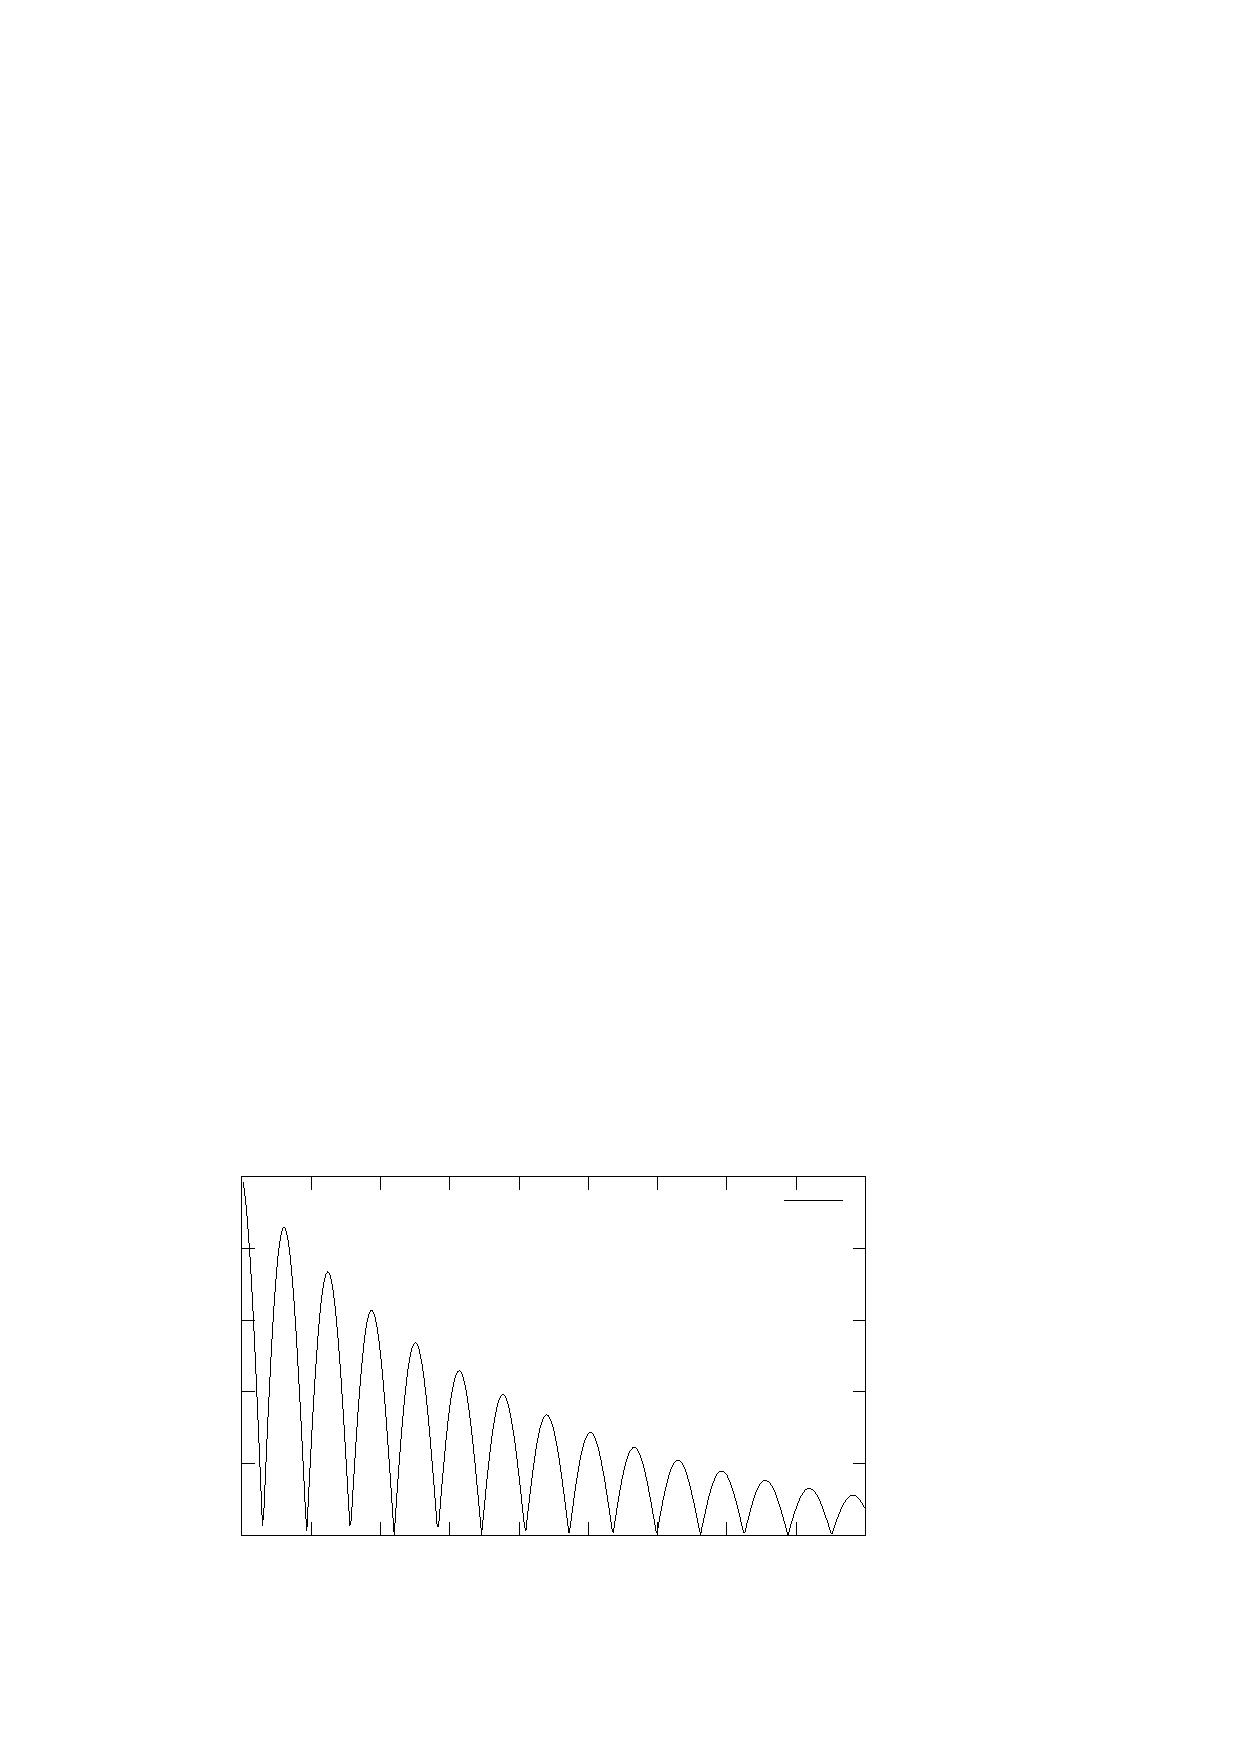
\includegraphics{diodes}%
\end{picture}%
\begingroup
\setlength{\unitlength}{0.0200bp}%
\begin{picture}(18000,10800)(0,0)%
\put(1925,1650){\makebox(0,0)[r]{\strut{} 0}}%
\put(1925,3370){\makebox(0,0)[r]{\strut{} 2}}%
\put(1925,5090){\makebox(0,0)[r]{\strut{} 4}}%
\put(1925,6810){\makebox(0,0)[r]{\strut{} 6}}%
\put(1925,8530){\makebox(0,0)[r]{\strut{} 8}}%
\put(1925,10250){\makebox(0,0)[r]{\strut{} 10}}%
\put(2200,1100){\makebox(0,0){\strut{} 0}}%
\put(3864,1100){\makebox(0,0){\strut{} 50}}%
\put(5528,1100){\makebox(0,0){\strut{} 100}}%
\put(7192,1100){\makebox(0,0){\strut{} 150}}%
\put(8856,1100){\makebox(0,0){\strut{} 200}}%
\put(10519,1100){\makebox(0,0){\strut{} 250}}%
\put(12183,1100){\makebox(0,0){\strut{} 300}}%
\put(13847,1100){\makebox(0,0){\strut{} 350}}%
\put(15511,1100){\makebox(0,0){\strut{} 400}}%
\put(17175,1100){\makebox(0,0){\strut{} 450}}%
\put(550,5950){\rotatebox{90}{\makebox(0,0){\strut{}U23}}}%
\put(9687,275){\makebox(0,0){\strut{}time e-5 s}}%
\put(14950,9675){\makebox(0,0)[r]{\strut{}'DiodeBridge.traj'}}%
\end{picture}%
\endgroup
\endinput

\caption{Diode bridges simulation}
\label{fig-Diode-sim}
\end {figure} 




\section{The Buck converter example}
\begin{figure}[h]
\centerline{
 \scalebox{1.0}{
    \input{buck.pstex_t}
 }
}
\caption{Buck converter}
\label{fig-Buck-converter}
\end{figure}
\subsection{Unknowns}
$x=^{t}(U_{45},U_{67},U_{08},I_{18}) Z_{s}=^{t}(V_{1},V_{2},V_{3},V_{4},V_{5},V_{6},V_{7},V_{8},V_{9},V_{10},I_{90},I_{20},I_{30},I_{100},I_{40})
Z_{ns}=^{t}(I_{1},I_{2},I_{3},I_{4},U_{2})$\\
\subsection{Matrices formulation}
\underline{To get $Ax'= Bx+CZ_{s}$}
\[\left(\begin{array}{c}
  \\
KCL(4)\\KCL(7)\\KCL(8)\\I_{18}
\end{array}\right)
\left(\begin{array}{cccc}
  U_{45}'&U_{67}'&U_{08}'&I_{18}'\\
  \hline
  C21&0&0&0\\
  0&-C11&0&0\\
  0&0&C&0\\
  0&0&0&L\\  
\end{array}\right)x'=
\left(\begin{array}{cccc}
  U_{45}&U_{67}&U_{08}&I_{18}\\
  \hline
  0&0&0&0\\
  0&0&0&0\\
  0&0&0&1\\
  0&0&0&0\\
\end{array}\right)x+\]
\[
\left(\begin{array}{ccccccccccccccc}
  V_{1}&V_{2}&V_{3}&V_{4}&V_{5}&V_{6}&V_{7}&V_{8}&V_{9}&V_{10}&I_{90}&I_{20}&I_{30}&I_{100}&I_{40}\\
  \hline
  0&0&0&0&0&0&0&0&0&0&0&0&0&0&-1\\
  0&0&0&0&0&0&-\frac{1}{R11}&\frac{1}{R11}&0&0&0&0&0&0&0\\
  0&0&0&0&0&\frac{1}{R12}&\frac{1}{R11}&\frac{-1}{Rload}-\frac{1}{R11}-\frac{1}{R12}&0&0&0&0&0&0&0\\
  1&0&0&0&0&0&0&0&0&0&0&0&0&0&0
\end{array}\right)Z_{s}+0Z_{ns}\]
\underline{To build the system $Ex+FZ_{s}+GZ_{ns}=s$}
\[
\left(\begin{array}{c}
  \\
KCL(1)\\KCL(2)\\KCL(3)\\KCL(5)\\KCL(6)\\KCL(9)\\KCL(10)\\VD_{100}\\VD_{2}\\VD_{30}\\VD_{90}\\VD_{40}\\U_{45}\\U_{67}\\U_{08}
\end{array}\right)
\left(\begin{array}{cccc}
  U_{45}&U_{67}&U_{08}&I_{18}\\
  \hline
  0&0&0&-1\\
  0&0&0&0\\
  0&0&0&0\\
  0&0&0&0\\
  0&0&0&0\\
  0&0&0&0\\
  0&0&0&0\\
  0&0&0&0\\
  0&0&0&0\\
  0&0&0&0\\
  0&0&0&0\\
  0&0&0&0\\
  1&0&0&0\\
  0&1&0&0\\
  0&0&1&0\\
\end{array}\right)x+\]
\[
\left(\begin{array}{ccccccccccccccc}
  V_{1}&V_{2}&V_{3}&V_{4}&V_{5}&V_{6}&V_{7}&V_{8}&V_{9}&V_{10}&I_{90}&I_{20}&I_{30}&I_{100}&I_{40}\\
  \hline
  0&0&0&0&0&0&0&0&0&0&0&0&0&0&0\\
  0&0&0&0&0&0&0&0&0&0&0&1&0&0&0\\
  0&0&0&0&0&0&0&0&0&0&0&0&1&0&0\\
  0&0&0&0&-\frac{1}{R21}&\frac{1}{R21}&0&0&0&0&0&0&0&0&-1\\
  0&0&0&0&\frac{1}{R21}&-\frac{1}{R12}-\frac{1}{R21}&\frac{1}{R11}&\frac{1}{R12}-\frac{1}{R11}&0&0&0&0&0&0&0\\
  0&0&0&0&0&0&0&0&0&0&1&0&0&0&0\\
  0&0&0&0&0&0&0&0&0&0&0&0&0&-1&0\\
  0&0&0&0&0&0&0&0&0&1&0&0&0&0&0\\
  0&1&0&0&0&0&0&0&0&0&0&0&0&0&0\\
  0&0&1&0&0&0&0&0&0&0&0&0&0&0&0\\
  0&0&0&0&0&0&0&0&1&0&0&0&0&0&0\\
  0&0&0&1&0&-G2&0&0&G2&0&0&0&0&0&0\\
  0&0&0&-1&1&0&0&0&0&0&0&0&0&0&0\\
  0&0&0&0&0&-1&1&0&0&0&0&0&0&0&0\\
  0&0&0&0&0&0&0&1&0&0&0&0&0&0&0\\
\end{array}\right)Z_{s}+\]
\[
\left(\begin{array}{ccccc}
  I_{1}&I_{2}&I_{3}&I_{4}&U_{2}\\
  \hline
  1&-1&-1&1&0\\
  0&0&0&0&0\\
  0&0&0&0&0\\
  0&0&0&0&0\\
  0&0&0&0&0\\
  0&0&0&0&0\\
  0&1&1&0&0\\
  0&0&0&0&0\\
  0&0&0&0&-1\\
  0&0&0&0&0\\
  0&0&0&0&0\\
  0&0&0&0&0\\
  0&0&0&0&0\\
  0&0&0&0&0\\
  0&0&0&0&0\\
\end{array}\right)Z_{ns}=
\left(\begin{array}{c}
  \\
0\\0\\0\\0\\0\\0\\0\\V1\\0\\Vramp\\Vref\\0\\0\\0\\0
\end{array}\right)\]
$N_{I}=N_{E}-4=24$
\newpage
And the non smooth equations:dim(Y)=dim($\lambda$ )=10.\\
\underline{$Z_{ns}=B\lambda$}\\
With B=
\tiny
\[
\left(\begin{array}{cccccccccccccccccccccccc}
0.09&0.2&0.4&1.1&2.8&-0.09&-0.2&-0.4&-1.1&-2.8&0&0&0&0&0&0&0&0&0&0&0&0&0&0\\
0&0&0&0&0&0&0&0&0&0&1&0&0&0&0&0&0&0&0&0&0&0&0&0\\
0&0&0&0&0&0&0&0&0&0&0&1&0&0&0&0&0&0&0&0&0&0&0&0\\
0&0&0&0&0&0&0&0&0&0&0&0&0.09&0.2&0.4&1.1&2.8&-0.09&-0.2&-0.4&-1.1&-2.8&0&0\\
0&0&0&0&0&0&0&0&0&0&0&0&0&0&0&0&0&0&0&0&0&0&25&-25
\end{array}\right)\]

\small
\underline{$Y=D\lambda$+Ex+s}
\[\left(\begin{array}{c}
  \\Y1\\Y2\\Y3\\Y4\\Y5\\Y6\\Y7\\Y8\\Y9\\Y10\\Y11\\Y12\\Y13\\Y14\\Y15\\Y16\\Y17\\Y18\\Y19\\Y20\\Y21\\Y22\\Y23\\Y24
 \end{array}\right)=
\left(\begin{array}{cccccccccccccccccccccccc}
  \\
  \hline
1&0&0&0&0&0&0&0&0&0&0&0&0&0&0&0&0&0&0&0&0&0&0&0\\
0&1&0&0&0&0&0&0&0&0&0&0&0&0&0&0&0&0&0&0&0&0&0&0\\
0&0&1&0&0&0&0&0&0&0&0&0&0&0&0&0&0&0&0&0&0&0&0&0\\
0&0&0&1&0&0&0&0&0&0&0&0&0&0&0&0&0&0&0&0&0&0&0&0\\
0&0&0&0&1&0&0&0&0&0&0&0&0&0&0&0&0&0&0&0&0&0&0&0\\
0&0&0&0&0&1&0&0&0&0&0&0&0&0&0&0&0&0&0&0&0&0&0&0\\
0&0&0&0&0&0&1&0&0&0&0&0&0&0&0&0&0&0&0&0&0&0&0&0\\
0&0&0&0&0&0&0&1&0&0&0&0&0&0&0&0&0&0&0&0&0&0&0&0\\
0&0&0&0&0&0&0&0&1&0&0&0&0&0&0&0&0&0&0&0&0&0&0&0\\
0&0&0&0&0&0&0&0&0&1&0&0&0&0&0&0&0&0&0&0&0&0&0&0\\
0&0&0&0&0&0&0&0&0&0&0&0&0&0&0&0&0&0&0&0&0&0&0&0\\
0&0&0&0&0&0&0&0&0&0&0&0&0&0&0&0&0&0&0&0&0&0&0&0\\
0&0&0&0&0&0&0&0&0&0&0&0&1&0&0&0&0&0&0&0&0&0&0&0\\
0&0&0&0&0&0&0&0&0&0&0&0&0&1&0&0&0&0&0&0&0&0&0&0\\
0&0&0&0&0&0&0&0&0&0&0&0&0&0&1&0&0&0&0&0&0&0&0&0\\
0&0&0&0&0&0&0&0&0&0&0&0&0&0&0&1&0&0&0&0&0&0&0&0\\
0&0&0&0&0&0&0&0&0&0&0&0&0&0&0&0&1&0&0&0&0&0&0&0\\
0&0&0&0&0&0&0&0&0&0&0&0&0&0&0&0&0&1&0&0&0&0&0&0\\
0&0&0&0&0&0&0&0&0&0&0&0&0&0&0&0&0&0&1&0&0&0&0&0\\
0&0&0&0&0&0&0&0&0&0&0&0&0&0&0&0&0&0&0&1&0&0&0&0\\
0&0&0&0&0&0&0&0&0&0&0&0&0&0&0&0&0&0&0&0&1&0&0&0\\
0&0&0&0&0&0&0&0&0&0&0&0&0&0&0&0&0&0&0&0&0&1&0&0\\
0&0&0&0&0&0&0&0&0&0&0&0&0&0&0&0&0&0&0&0&0&0&1&0\\
0&0&0&0&0&0&0&0&0&0&0&0&0&0&0&0&0&0&0&0&0&0&0&1
\end{array}\right)\lambda+\]
\[
\left(\begin{array}{ccccccccccccccc}
  V_{1}&V_{2}&V_{3}&V_{4}&V_{5}&V_{6}&V_{7}&V_{8}&V_{9}&V_{10}&I_{90}&I_{20}&I_{30}&I_{100}&I_{40}\\
  \hline
  0&-b&0&0&0&0&0&0&0&3&0&0&0&0&0\\
  0&-b&0&0&0&0&0&0&0&3&0&0&0&0&0\\
  0&-b&0&0&0&0&0&0&0&3&0&0&0&0&0\\
  0&-b&0&0&0&0&0&0&0&3&0&0&0&0&0\\
  0&-b&0&0&0&0&0&0&0&3&0&0&0&0&0\\
  b&-b&0&0&0&0&0&0&0&0&0&0&0&0&0\\
  b&-b&0&0&0&0&0&0&0&0&0&0&0&0&0\\
  b&-b&0&0&0&0&0&0&0&0&0&0&0&0&0\\
  b&-b&0&0&0&0&0&0&0&0&0&0&0&0&0\\
  b&-b&0&0&0&0&0&0&0&0&0&0&0&0&0\\
  1&0&0&0&0&0&0&0&0&0&0&0&0&0&0\\
  -1&0&0&0&0&0&0&0&0&1&0&0&0&0&0\\
  0&-b&0&0&0&0&0&0&0&3&0&0&0&0&0\\
  0&-b&0&0&0&0&0&0&0&3&0&0&0&0&0\\
  0&-b&0&0&0&0&0&0&0&3&0&0&0&0&0\\
  0&-b&0&0&0&0&0&0&0&3&0&0&0&0&0\\
  0&-b&0&0&0&0&0&0&0&3&0&0&0&0&0\\
  b&-b&0&0&0&0&0&0&0&0&0&0&0&0&0\\
  b&-b&0&0&0&0&0&0&0&0&0&0&0&0&0\\
  b&-b&0&0&0&0&0&0&0&0&0&0&0&0&0\\
  b&-b&0&0&0&0&0&0&0&0&0&0&0&0&0\\
  b&-b&0&0&0&0&0&0&0&0&0&0&0&0&0\\
  0&0&-1&1&0&0&0&0&0&0&0&0&0&0&0\\
  0&0&-1&1&0&0&0&0&0&0&0&0&0&0&0\\
\end{array}\right)Z_{s}=
\left(\begin{array}{c}
  \\h1\\h2\\h3\\h4\\h5\\h6\\h7\\h8\\h9\\h10\\0\\0\\h1\\h2\\h3\\h4\\h5\\h6\\h7\\h8\\h9\\h10\\-0.1\\0.1
  \end{array}\right)
  \]
\normalsize
\subsection{Simulation}

The simulation computed 4 million steps with a 50 ps fixed time step. The figure \ref{fig-Buck-sim} shows the inductor current of the circuit.

\begin {figure}[h]
%GNUPLOT: LaTeX picture with Postscript
\begin{picture}(0,0)%
\includegraphics{Buck}%
\end{picture}%
\begingroup
\setlength{\unitlength}{0.0200bp}%
\begin{picture}(18000,10800)(0,0)%
\put(2200,1650){\makebox(0,0)[r]{\strut{}-0.7}}%
\put(2200,2725){\makebox(0,0)[r]{\strut{}-0.6}}%
\put(2200,3800){\makebox(0,0)[r]{\strut{}-0.5}}%
\put(2200,4875){\makebox(0,0)[r]{\strut{}-0.4}}%
\put(2200,5950){\makebox(0,0)[r]{\strut{}-0.3}}%
\put(2200,7025){\makebox(0,0)[r]{\strut{}-0.2}}%
\put(2200,8100){\makebox(0,0)[r]{\strut{}-0.1}}%
\put(2200,9175){\makebox(0,0)[r]{\strut{} 0}}%
\put(2200,10250){\makebox(0,0)[r]{\strut{} 0.1}}%
\put(2475,1100){\makebox(0,0){\strut{}   0}}%
\put(3945,1100){\makebox(0,0){\strut{}   2e-5}}%
\put(5415,1100){\makebox(0,0){\strut{}   4e-5}}%
\put(6885,1100){\makebox(0,0){\strut{}   6e-5}}%
\put(8355,1100){\makebox(0,0){\strut{}   8e-5}}%
\put(9825,1100){\makebox(0,0){\strut{}   1e-4}}%
\put(11295,1100){\makebox(0,0){\strut{}   1.2e-4}}%
\put(12765,1100){\makebox(0,0){\strut{}   1.4e-4}}%
\put(14235,1100){\makebox(0,0){\strut{}   1.6e-4}}%
\put(15705,1100){\makebox(0,0){\strut{}   1.8e-4}}%
\put(17175,1100){\makebox(0,0){\strut{}   2e-4}}%
\put(550,5950){\rotatebox{90}{\makebox(0,0){\strut{}Inductor current}}}%
\put(9825,275){\makebox(0,0){\strut{}time s}}%
\end{picture}%
\endgroup
\endinput

\caption{Buck simulation}
\label{fig-Buck-sim}
\end {figure} 
\newpage
%*************************************OTHER ANALYSIS

%EXAMPLE SECTION************************************************************************************



\section{Conclusion}
This document demonstrates a way to develop an automatic circuit equation formulation. It shows that a Moreau's time
stepping lead to a MLCP. The previous examples describe the method with non smooth circuits.


%%% Local Variables: 
%%% mode: latex
%%% TeX-master: "ace"
%%% End: 
